\documentclass[a4paper]{book}
\usepackage{makeidx}
\usepackage{graphicx}
\usepackage{multicol}
\usepackage{float}
\usepackage{listings}
\usepackage{color}
\usepackage{ifthen}
\usepackage[table]{xcolor}
\usepackage{textcomp}
\usepackage{alltt}
\usepackage{ifpdf}
\ifpdf
\usepackage[pdftex,
            pagebackref=true,
            colorlinks=true,
            linkcolor=blue,
            unicode
           ]{hyperref}
\else
\usepackage[ps2pdf,
            pagebackref=true,
            colorlinks=true,
            linkcolor=blue,
            unicode
           ]{hyperref}
\usepackage{pspicture}
\fi
\usepackage[utf8]{inputenc}
\usepackage{mathptmx}
\usepackage[scaled=.90]{helvet}
\usepackage{courier}
\usepackage{sectsty}
\usepackage[titles]{tocloft}
\usepackage{doxygen}
\lstset{language=C++,inputencoding=utf8,basicstyle=\footnotesize,breaklines=true,breakatwhitespace=true,tabsize=8,numbers=left }
\makeindex
\setcounter{tocdepth}{3}
\renewcommand{\footrulewidth}{0.4pt}
\renewcommand{\familydefault}{\sfdefault}
\begin{document}
\hypersetup{pageanchor=false}
\begin{titlepage}
\vspace*{7cm}
\begin{center}
{\Large Reference Manual}\\
\vspace*{1cm}
{\large Generated by Doxygen 1.7.4}\\
\vspace*{0.5cm}
{\small Wed Feb 15 2012 03:45:09}\\
\end{center}
\end{titlepage}
\clearemptydoublepage
\pagenumbering{roman}
\tableofcontents
\clearemptydoublepage
\pagenumbering{arabic}
\hypersetup{pageanchor=true}
\chapter{Class Index}
\section{Class List}
Here are the classes, structs, unions and interfaces with brief descriptions:\begin{DoxyCompactList}
\item\contentsline{section}{\hyperlink{structcgpa}{cgpa} }{\pageref{structcgpa}}{}
\item\contentsline{section}{\hyperlink{structchoice}{choice} }{\pageref{structchoice}}{}
\end{DoxyCompactList}

\chapter{File Index}
\section{File List}
Here is a list of all files with brief descriptions:\begin{DoxyCompactList}
\item\contentsline{section}{code/\hyperlink{allocation_8c}{allocation.c} }{\pageref{allocation_8c}}{}
\end{DoxyCompactList}

\chapter{Class Documentation}
\hypertarget{structcgpa}{
\section{cgpa Struct Reference}
\label{structcgpa}\index{cgpa@{cgpa}}
}
\subsection*{Public Attributes}
\begin{DoxyCompactItemize}
\item 
char \hyperlink{structcgpa_a4d971d968022affbe8670220fea9c34b}{name} \mbox{[}MAX\_\-NAME\_\-LEN\mbox{]}
\item 
char \hyperlink{structcgpa_a9863e09e4c26b3f711707ec894044031}{dept} \mbox{[}4\mbox{]}
\item 
float \hyperlink{structcgpa_aeae583a9994da725e72120846f307087}{marks}
\end{DoxyCompactItemize}


\subsection{Detailed Description}
struct to hold cgpa info 

Definition at line 19 of file allocation.c.



\subsection{Member Data Documentation}
\hypertarget{structcgpa_a9863e09e4c26b3f711707ec894044031}{
\index{cgpa@{cgpa}!dept@{dept}}
\index{dept@{dept}!cgpa@{cgpa}}
\subsubsection[{dept}]{\setlength{\rightskip}{0pt plus 5cm}char {\bf cgpa.dept}\mbox{[}4\mbox{]}}}
\label{structcgpa_a9863e09e4c26b3f711707ec894044031}


Definition at line 21 of file allocation.c.

\hypertarget{structcgpa_aeae583a9994da725e72120846f307087}{
\index{cgpa@{cgpa}!marks@{marks}}
\index{marks@{marks}!cgpa@{cgpa}}
\subsubsection[{marks}]{\setlength{\rightskip}{0pt plus 5cm}float {\bf cgpa.marks}}}
\label{structcgpa_aeae583a9994da725e72120846f307087}


Definition at line 22 of file allocation.c.

\hypertarget{structcgpa_a4d971d968022affbe8670220fea9c34b}{
\index{cgpa@{cgpa}!name@{name}}
\index{name@{name}!cgpa@{cgpa}}
\subsubsection[{name}]{\setlength{\rightskip}{0pt plus 5cm}char {\bf cgpa.name}\mbox{[}MAX\_\-NAME\_\-LEN\mbox{]}}}
\label{structcgpa_a4d971d968022affbe8670220fea9c34b}


Definition at line 20 of file allocation.c.



The documentation for this struct was generated from the following file:\begin{DoxyCompactItemize}
\item 
code/\hyperlink{allocation_8c}{allocation.c}\end{DoxyCompactItemize}

\hypertarget{structchoice}{
\section{choice Struct Reference}
\label{structchoice}\index{choice@{choice}}
}
\subsection*{Public Attributes}
\begin{DoxyCompactItemize}
\item 
char \hyperlink{structchoice_a6385591a8684ca883a69f2ef18ec0a5b}{name} \mbox{[}MAX\_\-NAME\_\-LEN\mbox{]}
\item 
char \hyperlink{structchoice_a261d0ea7417aa775dc50cb0d8c358cce}{choice} \mbox{[}11\mbox{]}\mbox{[}4\mbox{]}
\end{DoxyCompactItemize}


\subsection{Detailed Description}
struct to hold choice info 

Definition at line 50 of file allocation.c.



\subsection{Member Data Documentation}
\hypertarget{structchoice_a261d0ea7417aa775dc50cb0d8c358cce}{
\index{choice@{choice}!choice@{choice}}
\index{choice@{choice}!choice@{choice}}
\subsubsection[{choice}]{\setlength{\rightskip}{0pt plus 5cm}char {\bf choice.choice}\mbox{[}11\mbox{]}\mbox{[}4\mbox{]}}}
\label{structchoice_a261d0ea7417aa775dc50cb0d8c358cce}


Definition at line 52 of file allocation.c.

\hypertarget{structchoice_a6385591a8684ca883a69f2ef18ec0a5b}{
\index{choice@{choice}!name@{name}}
\index{name@{name}!choice@{choice}}
\subsubsection[{name}]{\setlength{\rightskip}{0pt plus 5cm}char {\bf choice.name}\mbox{[}MAX\_\-NAME\_\-LEN\mbox{]}}}
\label{structchoice_a6385591a8684ca883a69f2ef18ec0a5b}


Definition at line 51 of file allocation.c.



The documentation for this struct was generated from the following file:\begin{DoxyCompactItemize}
\item 
code/\hyperlink{allocation_8c}{allocation.c}\end{DoxyCompactItemize}

\chapter{File Documentation}
\hypertarget{allocation_8c}{
\section{code/allocation.c File Reference}
\label{allocation_8c}\index{code/allocation.c@{code/allocation.c}}
}
{\ttfamily \#include $<$errno.h$>$}\par
{\ttfamily \#include $<$getopt.h$>$}\par
{\ttfamily \#include $<$stdio.h$>$}\par
{\ttfamily \#include $<$stdlib.h$>$}\par
{\ttfamily \#include $<$string.h$>$}\par
{\ttfamily \#include $<$ncurses.h$>$}\par
{\ttfamily \#include $<$sys/queue.h$>$}\par
Include dependency graph for allocation.c:
\nopagebreak
\begin{figure}[H]
\begin{center}
\leavevmode
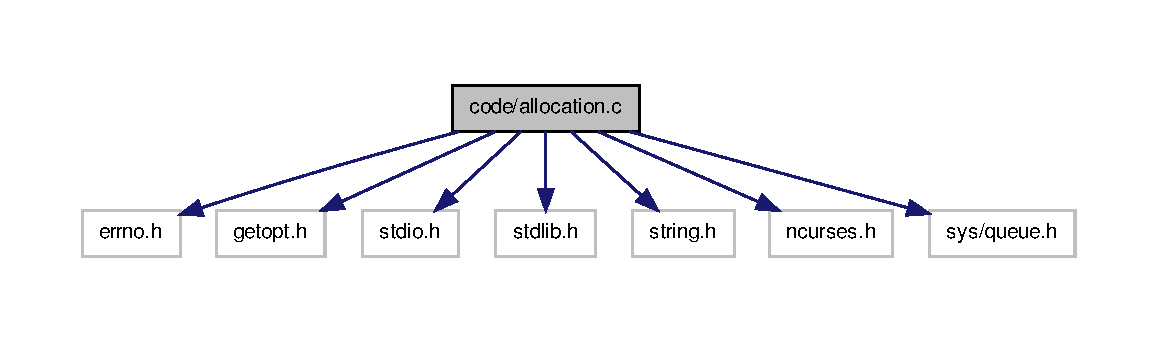
\includegraphics[width=400pt]{allocation_8c__incl}
\end{center}
\end{figure}
\subsection*{Classes}
\begin{DoxyCompactItemize}
\item 
struct \hyperlink{structcgpa}{cgpa}
\item 
struct \hyperlink{structchoice}{choice}
\end{DoxyCompactItemize}
\subsection*{Defines}
\begin{DoxyCompactItemize}
\item 
\#define \hyperlink{allocation_8c_afd709f201d7643c3909621f620ea648a}{MAX\_\-NAME\_\-LEN}~50
\end{DoxyCompactItemize}
\subsection*{Functions}
\begin{DoxyCompactItemize}
\item 
int \hyperlink{allocation_8c_a3c04138a5bfe5d72780bb7e82a18e627}{main} (int argc, char $\ast$$\ast$argv)
\end{DoxyCompactItemize}


\subsection{Define Documentation}
\hypertarget{allocation_8c_afd709f201d7643c3909621f620ea648a}{
\index{allocation.c@{allocation.c}!MAX\_\-NAME\_\-LEN@{MAX\_\-NAME\_\-LEN}}
\index{MAX\_\-NAME\_\-LEN@{MAX\_\-NAME\_\-LEN}!allocation.c@{allocation.c}}
\subsubsection[{MAX\_\-NAME\_\-LEN}]{\setlength{\rightskip}{0pt plus 5cm}\#define MAX\_\-NAME\_\-LEN~50}}
\label{allocation_8c_afd709f201d7643c3909621f620ea648a}
This program will implement a trick of card as stated in the assignment problem. 

Definition at line 14 of file allocation.c.



\subsection{Function Documentation}
\hypertarget{allocation_8c_a3c04138a5bfe5d72780bb7e82a18e627}{
\index{allocation.c@{allocation.c}!main@{main}}
\index{main@{main}!allocation.c@{allocation.c}}
\subsubsection[{main}]{\setlength{\rightskip}{0pt plus 5cm}int main (
\begin{DoxyParamCaption}
\item[{int}]{argc, }
\item[{char $\ast$$\ast$}]{argv}
\end{DoxyParamCaption}
)}}
\label{allocation_8c_a3c04138a5bfe5d72780bb7e82a18e627}
Main function of program reads input file and then implement the algorithm described in design document. 

Definition at line 524 of file allocation.c.


\printindex
\end{document}
